% Shared preamble of the six stage reports (stages/README.md). Colours and notation are identical in every report.
\documentclass[11pt,a4paper]{article}
\usepackage[margin=2.2cm]{geometry}
\usepackage{amsmath,amssymb,booktabs,graphicx,xcolor,float,caption,subcaption,enumitem,longtable,array}
\usepackage[round]{natbib}
\usepackage[hidelinks]{hyperref}
\usepackage{fancyhdr}
\setlength{\emergencystretch}{2em}
\setlength{\parskip}{3pt}
\definecolor{roigreen}{RGB}{0,160,0}
\definecolor{artred}{RGB}{220,0,0}
\definecolor{maskblue}{RGB}{31,119,180}
\definecolor{ermgrey}{RGB}{110,110,110}
\definecolor{supported}{RGB}{0,120,0}
\definecolor{notsupported}{RGB}{190,0,0}
\newcommand{\ok}{\textcolor{supported}{\textbf{supported}}}
\newcommand{\no}{\textcolor{notsupported}{\textbf{not supported}}}
\newcommand{\mixed}{\textcolor{orange!80!black}{\textbf{partly supported}}}
\newcommand{\roi}{\textcolor{roigreen}{ROI}}
\newcommand{\na}{\textit{n/a}}
\newcommand{\registered}[1]{\textsf{registered before results (#1)}}
\newcommand{\posthoc}[1]{\textsf{post hoc (#1)}}
\pagestyle{fancy}\fancyhf{}\rhead{\small Where the Shortcut Sits --- stage reports}\lfoot{\small\leftmark}\rfoot{\small\thepage}
\newcommand{\stagebox}[1]{\noindent\colorbox{gray!12}{\parbox{\dimexpr\linewidth-2\fboxsep}{\small #1}}\par\medskip}

% generated by make_stage*.py from result files; do not edit
\providecommand{\sFiveNatthyroidall}{$-0.004$ [$-0.048, +0.041$]}
\providecommand{\sFiveNatthyroidhard}{$-0.095$ [$-0.165, -0.022$]}
\providecommand{\sFiveNatthyroideasy}{$+0.042$ [$-0.011, +0.097$]}
\providecommand{\sFiveNatisicBCNall}{$-0.025$ [$-0.035, -0.016$]}
\providecommand{\sFiveNatisicBCNhard}{$-0.025$ [$-0.043, -0.008$]}
\providecommand{\sFiveNatisicBCNeasy}{$-0.022$ [$-0.035, -0.008$]}
\providecommand{\sFiveNatisicHAMall}{$+0.031$ [$+0.017, +0.045$]}
\providecommand{\sFiveNatisicHAMhard}{$+0.050$ [$+0.030, +0.070$]}
\providecommand{\sFiveNatisicHAMeasy}{$+0.004$ [$-0.019, +0.027$]}
\providecommand{\sFiveNatisicMSKall}{$+0.016$ [$-0.007, +0.038$]}
\providecommand{\sFiveNatisicMSKhard}{$-0.065$ [$-0.111, -0.019$]}
\providecommand{\sFiveNatisicMSKeasy}{$+0.100$ [$+0.056, +0.147$]}
\providecommand{\sFiveNatcapsuleall}{$+0.077$ [$+0.059, +0.097$]}
\providecommand{\sFiveNatcapsulehard}{$+0.021$ [$-0.003, +0.048$]}
\providecommand{\sFiveNatcapsuleeasy}{$+0.071$ [$+0.040, +0.108$]}
\providecommand{\sFiveThyAucerm}{0.735}
\providecommand{\sFiveThySenserm}{0.699}
\providecommand{\sFiveThySpecerm}{0.653}
\providecommand{\sFiveThyAucmask}{0.731}
\providecommand{\sFiveThySensmask}{0.424}
\providecommand{\sFiveThySpecmask}{0.856}
\providecommand{\sFiveSensOPOne}{$-0.275$ [$-0.435, -0.138$]}
\providecommand{\sFiveConfOPOne}{$-0.479$ [$-0.640, -0.313$]}
\providecommand{\sFiveConfErmOPOne}{0.703}
\providecommand{\sFiveConfMaskOPOne}{0.223}
\providecommand{\sFiveSensOPTwo}{$-0.202$ [$-0.300, -0.100$]}
\providecommand{\sFiveConfOPTwo}{$-0.372$ [$-0.499, -0.236$]}
\providecommand{\sFiveConfErmOPTwo}{0.549}
\providecommand{\sFiveConfMaskOPTwo}{0.177}
\providecommand{\sFiveSensOPThree}{$-0.152$ [$-0.253, -0.043$]}
\providecommand{\sFiveConfOPThree}{$-0.236$ [$-0.383, -0.089$]}
\providecommand{\sFiveConfErmOPThree}{0.336}
\providecommand{\sFiveConfMaskOPThree}{0.100}
\providecommand{\sFiveSensOPFour}{$-0.373$ [$-0.469, -0.270$]}
\providecommand{\sFiveConfOPFour}{$-0.546$ [$-0.671, -0.421$]}
\providecommand{\sFiveConfErmOPFour}{0.744}
\providecommand{\sFiveConfMaskOPFour}{0.197}
\providecommand{\sFiveSensOPFive}{$-0.281$ [$-0.391, -0.178$]}
\providecommand{\sFiveConfOPFive}{$-0.462$ [$-0.614, -0.310$]}
\providecommand{\sFiveConfErmOPFive}{0.862}
\providecommand{\sFiveConfMaskOPFive}{0.400}
\providecommand{\sFiveNConf}{78}
\providecommand{\sFiveNSensLoss}{4}
\providecommand{\sFiveFtDermoscopyhairResNetFiveZero}{$+0.143$ [$+0.054, +0.232$]}
\providecommand{\sFiveFtThyroidResNetFiveZero}{$+0.063$ [$-0.022, +0.144$]}
\providecommand{\sFiveFtThyroidViTS}{$+0.122$ [$+0.039, +0.211$]}
\providecommand{\sFiveFtCapsuleResNetFiveZero}{$+0.606$ [$+0.495, +0.716$]}
\providecommand{\sFiveFtOvaryResNetFiveZeroOneFiveclusters}{$+0.058$ [$-0.062, +0.179$]}
\providecommand{\sFiveNBreadth}{24}
\providecommand{\sFiveNFrozen}{18}
\providecommand{\sFiveNFrozenPos}{17}
\providecommand{\sFiveNFt}{5}
\providecommand{\sFiveNFtPos}{3}
\providecommand{\sFiveExtX}{$+0.250$ [$+0.174, +0.327$]}
\providecommand{\sFiveExttrapA}{$-0.064$ [$-0.128, -0.002$]}
\providecommand{\sFiveExttrapB}{$+0.186$ [$+0.118, +0.249$]}
\providecommand{\sFiveExtPatients}{2,056}
\providecommand{\sFiveExtImages}{32,997}
\providecommand{\sFiveExtMel}{583}
\providecommand{\sFiveDermmasktrapAtestrev}{$-0.104$ [$-0.143, -0.067$]}
\providecommand{\sFiveDermmasktrapAclean}{$-0.066$ [$-0.089, -0.043$]}
\providecommand{\sFiveDerminpainttrapAtestrev}{$+0.033$ [$+0.025, +0.042$]}
\providecommand{\sFiveDerminpainttrapAclean}{$+0.011$ [$+0.005, +0.017$]}
\providecommand{\sFiveDermbalancedtrapAtestrev}{$+0.146$ [$+0.122, +0.170$]}
\providecommand{\sFiveDermbalancedtrapAclean}{$+0.035$ [$+0.020, +0.050$]}
\providecommand{\sFiveDermmasktrapBtestrev}{$-0.090$ [$-0.135, -0.046$]}
\providecommand{\sFiveDermmasktrapBclean}{$-0.063$ [$-0.094, -0.033$]}
\providecommand{\sFiveDerminpainttrapBtestrev}{$+0.040$ [$+0.015, +0.064$]}
\providecommand{\sFiveDerminpainttrapBclean}{$+0.027$ [$+0.015, +0.039$]}
\providecommand{\sFiveDermbalancedtrapBtestrev}{$+0.110$ [$+0.089, +0.132$]}
\providecommand{\sFiveDermbalancedtrapBclean}{$+0.049$ [$+0.035, +0.063$]}
\providecommand{\sFiveDermPred}{+0.013}
\providecommand{\sFiveDermObs}{+0.014}
\providecommand{\sFiveTMae}{0.052}
\providecommand{\sFiveTMaeSym}{0.129}
\providecommand{\sFiveTMaeClean}{0.237}
\providecommand{\sFiveTR}{0.914}
\providecommand{\sFiveTN}{136}
\providecommand{\sFiveTWithin}{66\%}
\providecommand{\sFiveTTwoN}{9}
\providecommand{\sFiveTTwoSign}{9}
\providecommand{\sFiveTTwoMae}{0.015}
\providecommand{\sFiveTTwoR}{0.999}
\providecommand{\sFiveTTwoFt}{3/3}
\providecommand{\sFiveTThreeN}{50}
\providecommand{\sFiveTThreeSign}{44}
\providecommand{\sFiveTThreeMae}{0.057}
\providecommand{\sFiveTThreeSymSign}{38}
\providecommand{\sFiveTFourN}{9}
\providecommand{\sFiveTFourAgree}{8}
\providecommand{\sFiveTFtMae}{0.027}
\providecommand{\sFiveRegNat}{\texttt{74bd243}, 2026-09-27 09:39}
\providecommand{\sFiveRegRevTwo}{\texttt{29cd0da}, 2026-09-27 18:56}
\providecommand{\sFiveRegRevThree}{\texttt{85da735}, 2026-09-27 23:43}
\providecommand{\sFiveRegTheory}{\texttt{4f78653}, 2026-09-27 13:46}
\providecommand{\sFiveRegScale}{\texttt{13303b0}, 2026-09-27 14:13}
\providecommand{\sFiveRegFt}{\texttt{7c8b466}, 2026-09-27 07:06}
\providecommand{\sFiveRegFinal}{\texttt{c45d482}, 2026-09-28 00:35}
\providecommand{\sFiveRegIsic}{\texttt{76e25d4}, 2026-09-26 13:14}
\providecommand{\sFiveZsthyroid}{$+0.103$ [$+0.064, +0.143$]}
\providecommand{\sFiveZsGapthyroid}{$+0.072$}
\providecommand{\sFiveZsCleanthyroid}{0.451}
\providecommand{\sFiveZsovary}{$+0.181$ [$+0.103, +0.261$]}
\providecommand{\sFiveZsGapovary}{$-0.126$}
\providecommand{\sFiveZsCleanovary}{0.623}
\providecommand{\sFiveZscapsule}{$+0.045$ [$+0.001, +0.090$]}
\providecommand{\sFiveZsGapcapsule}{$-0.402$}
\providecommand{\sFiveZsCleancapsule}{0.631}
\providecommand{\sFiveZsisic}{$+0.040$ [$+0.021, +0.058$]}
\providecommand{\sFiveZsGapisic}{$+0.082$}
\providecommand{\sFiveZsCleanisic}{0.697}
\providecommand{\sFiveFtADermoscopyhairResNetFiveZero}{$-0.002$ [$-0.054, +0.049$]}
\providecommand{\sFiveFtBDermoscopyhairResNetFiveZero}{$+0.141$ [$+0.071, +0.214$]}
\providecommand{\sFiveFtAThyroidResNetFiveZero}{$+0.078$ [$+0.032, +0.123$]}
\providecommand{\sFiveFtBThyroidResNetFiveZero}{$+0.142$ [$+0.073, +0.211$]}
\providecommand{\sFiveFtAThyroidViTSOneSix}{$+0.122$ [$+0.068, +0.170$]}
\providecommand{\sFiveFtBThyroidViTSOneSix}{$+0.244$ [$+0.163, +0.329$]}
\providecommand{\sFiveFtACapsuleResNetFiveZero}{$-0.279$ [$-0.377, -0.185$]}
\providecommand{\sFiveFtBCapsuleResNetFiveZero}{$+0.327$ [$+0.235, +0.416$]}
\providecommand{\sFiveFtAOvaryResNetFiveZero}{$+0.152$ [$+0.070, +0.232$]}
\providecommand{\sFiveFtBOvaryResNetFiveZero}{$+0.211$ [$+0.090, +0.328$]}
\providecommand{\sFiveGapthyroidViTS}{0.537}
\providecommand{\sFiveGapthyroidViTB}{0.590}
\providecommand{\sFiveGapthyroidViTL}{0.622}
\providecommand{\sFiveGapovaryViTS}{0.320}
\providecommand{\sFiveGapovaryViTB}{0.413}
\providecommand{\sFiveGapovaryViTL}{0.564}
\providecommand{\sFiveGapcapsuleViTS}{0.363}
\providecommand{\sFiveGapcapsuleViTB}{0.360}
\providecommand{\sFiveGapcapsuleViTL}{0.347}
\providecommand{\sFiveLitOurs}{0.735}
\providecommand{\sFiveNatBalthyroidall}{$-0.017$ [$-0.065, +0.030$]}
\providecommand{\sFiveNatBalthyroidhard}{$+0.136$ [$+0.063, +0.207$]}
\providecommand{\sFiveNatBalisicBCNall}{$+0.022$ [$+0.012, +0.031$]}
\providecommand{\sFiveNatBalisicBCNhard}{$+0.043$ [$+0.026, +0.059$]}
\providecommand{\sFiveNatBalisicHAMall}{$-0.032$ [$-0.049, -0.013$]}
\providecommand{\sFiveNatBalisicHAMhard}{$-0.018$ [$-0.041, +0.007$]}
\providecommand{\sFiveNatBalisicMSKall}{$-0.018$ [$-0.041, +0.005$]}
\providecommand{\sFiveNatBalisicMSKhard}{$+0.100$ [$+0.055, +0.144$]}
\providecommand{\sFiveNatBalcapsuleall}{$-0.086$ [$-0.110, -0.065$]}
\providecommand{\sFiveNatBalcapsulehard}{$-0.009$ [$-0.035, +0.015$]}
\providecommand{\sFiveSimN}{29}
\providecommand{\sFiveSimMax}{0.009}
\providecommand{\sFiveOvFtCleanA}{0.60}
\providecommand{\sFiveOvFtCleanB}{0.50}
\providecommand{\sFiveEstN}{148}
\providecommand{\sFiveEstLost}{12}
\providecommand{\sFiveEstGained}{1}
\providecommand{\sFiveEstMed}{1.53}

\title{\textbf{Stage 5 --- Practice and theory}\\[3pt]\large Where the Shortcut Sits: supervisor meeting 5 of 6}
\author{}
\date{Report generated from the repository on \today}
\begin{document}
\maketitle
\stagebox{\textbf{In one sentence.} On unaltered test sets masking harms exactly the cases the location law says it
should --- shortcut-conflicting images with an in-ROI artifact --- and on the patient-disjoint thyroid split it lowers
sensitivity at every validation-fixed operating point; the crossover replicates in \sFiveNFrozenPos{} of
\sFiveNFrozen{} frozen encoder--cohort pairs, in \sFiveNFtPos{} of \sFiveNFt{} fine-tuned networks and on new patients
(ISIC 2020, \sFiveExtX); a two-parameter theory predicts held-out reversed AUROC with mean error \sFiveTMae, less than
half the error of the best heuristic.}
% Shared notation. Each stage defines \notY, \notA, \notROI, \notCross, \notCI and \notExtra before \input-ing this
% file, so that a report only names the cohorts and quantities it has already introduced.
\section*{Notation}
\begin{tabular}{p{3.2cm}p{11.8cm}}
$Y\in\{0,1\}$ & diagnosis: \notY. \\
$A\in\{0,1\}$ & artifact present: \notA. \\
ROI & region of interest: \notROI; drawn in \textcolor{roigreen}{green}; artifacts in \textcolor{artred}{red}. \\
$r$ & overlap $|\text{artifact}\cap\text{ROI}|/|\text{artifact}|$. Trap~A: $r\ge0.5$ (artifact in the ROI); Trap~B: $r<0.1$ (outside). \\
Environments & training and correlated test $P(A{=}1\mid Y{=}1)=0.9$, $P(A{=}1\mid Y{=}0)=0.1$; reversed test 0.1/0.9; clean test: artifact independent of $Y$ (real artifacts: half of each class) or absent (synthetic artifacts). \\
ERM, mask & linear head on the frozen features of the original image / of the ROI-masked image. \\
Crossover & \notCross \\
CI & \notCI \\
$|\Delta p|$ & same-head counterfactual sensitivity: change of the predicted probability when the artifact is inserted into the same image. \\
\notExtra
\end{tabular}


\section{Where we are}
Stages~2--4 established the location law in constructed environments --- a strong artifact--label correlation in
training and its reversal at test --- and showed that it is not explained by measured confounders. A clinician will ask
two questions this cannot answer: does it matter on data as it is collected, without an imposed correlation, and at
the operating point a clinic would use? And is the result a property of one encoder, or something that can be
predicted? This meeting answers both, reports the breadth of replication (encoder families and sizes, fine-tuning, new
patients), and explains the one encoder that does not show the crossover.

\section{Question}
\begin{enumerate}[label=\textbf{Q5\alph*},leftmargin=*]\itemsep1pt
\item On natural test sets, does masking harm the shortcut-conflicting cases, and does that change clinical
sensitivity at fixed operating points?
\item How broadly does the crossover replicate?
\item Can a simple model predict, before seeing it, how a model will perform on the reversed test --- and so explain
when masking helps?
\end{enumerate}
\paragraph{Design decisions} \emph{Hard pairs.} On a natural test set the artifact--label association is weak, so the
overall AUROC barely moves. We therefore split positive--negative pairs by whether their artifact status conflicts with
the test set's own association (``hard'') or follows it (``easy''); the law predicts harm on hard pairs.
\emph{Operating points fixed on validation data} (never on test) at five clinically motivated targets, with thresholds
re-estimated in every bootstrap replicate. \emph{Theory judged by held-out error}, not by fit: the model is fitted to
each cell's clean and correlated AUROC and must predict the reversed AUROC it never saw, against two parameter-free
heuristics. Rejected: judging the theory by agreement with simulations drawn from its own assumptions (circular).

\section{Methods}
\paragraph{Natural test sets} Thyroid: the official patient-disjoint TNCD test split \citep{gong2022acl}; dermoscopy: each
source (BCN, HAM, MSK) held out in turn; capsule: held-out frame blocks. Models are trained on the natural training
distribution (no imposed correlation). \paragraph{Clinical metrics and operating points} AUROC, AUPRC, Brier score,
expected calibration error; sensitivity and specificity at OP1 (maximal balanced accuracy), OP2/OP3 (validation
specificity $\ge0.80/0.90$) and OP4/OP5 (validation sensitivity $\ge0.80/0.90$), overall and among shortcut-conflicting
positives. \paragraph{Replication} DINOv2 ViT-S/B/L, MedSigLIP-448, ConvNeXt-384 and DermLIP (frozen, linear heads);
ResNet-50 and ViT-S fine-tuned end to end; ISIC 2020 as an external dermoscopy cohort with patient-disjoint folds.
\paragraph{Theory} A linear-Gaussian model with disease signal-to-noise $S$ and artifact signal-to-noise $A$, an
LDA-optimal head and the trap's training association predicts the AUROC of any test composition (\texttt{docs/THEORY.md}).
Per cell, $(S, A)$ is fitted to the clean and correlated AUROC; the reversed AUROC is predicted. Heuristics:
``reversed = clean'' and ``symmetric reversal'' (reversed $=$ clean $-$ (correlated $-$ clean)).

\section{Experiments}
\begin{table}[H]\centering\scriptsize
\caption{Experiments of this stage and their registration documents (\texttt{docs/PREREGISTRATION\_<name>.md}). Commit times are set by the committing machine and are not independent proof of order.}\label{tab:exp}
\begin{tabular}{p{3.1cm}p{2.1cm}p{2.4cm}p{3.2cm}p{3.3cm}}\toprule
Experiment & Status & Registration & First commit (local time) & Support criterion \\\midrule
Zero-shot vision--language scores, Z1 & \mixed{} registered (descriptive); crossover test post hoc & TEXT\_\allowbreak{}PROMPT & \texttt{7877e8c}, 2026-09-27 12:21 & correlated $-$ reversed gap reported \\
Natural test sets, N3 (hard pairs) & \ok{} registered & NATURAL & \texttt{74bd243}, 2026-09-27 09:39 & mask $-$ ERM $<0$ on hard pairs \\
Operating points S1--S3 & \ok{} registered & REVIEW2 (R3) & \texttt{29cd0da}, 2026-09-27 18:56 & ``masking lowers sensitivity'' only if S1 and $\ge3$ of OP2--OP5 \\
Thyroid subgroup, $n=$\sFiveNConf{} (S3) & \mixed{} registered test in a post hoc subgroup & REVIEW2 (R3) & \texttt{29cd0da}, 2026-09-27 18:56 & sensitivity loss in the subgroup, CI $<0$ \\
Crossed CIs for the subgroup (R6) & \ok{} registered & REVIEW3 (R6) & \texttt{85da735}, 2026-09-27 23:43 & report the crossed CI \\
Fine-tuned hair model and literature comparison (R4) & \ok{} registered & REVIEW2 (R4) & \texttt{29cd0da}, 2026-09-27 18:56 & crossover CI $>0$; comparison descriptive \\
Encoder scale (S/B/L) & \ok{} registered & SCALE & \texttt{13303b0}, 2026-09-27 14:13 & crossover CI $>0$ at every scale \\
Fine-tuned networks & \ok{} registered & FINETUNE & \texttt{7c8b466}, 2026-09-27 07:06 & crossover CI $>0$ (secondary) \\
DermLIP hair traps & \ok{} registered & ISIC2019\_\allowbreak{}TRAPS & \texttt{76e25d4}, 2026-09-26 13:14 & crossover CI $>0$ \\
Theory as held-out predictor, T1--T4 & \ok{} registered & THEORY\_\allowbreak{}PREDICTION & \texttt{4f78653}, 2026-09-27 13:46 & MAE below both heuristics; crossover signs \\
External validation, X1 (ISIC 2020) & \ok{} registered & FINAL (A4) & \texttt{c45d482}, 2026-09-28 00:35 & gate, then crossover CI $>0$ \\
\bottomrule\end{tabular}
\end{table}


\section{Results}
\subsection{Natural test sets}
Table~\ref{tab:nat}. On all pairs, masking changes little. On shortcut-conflicting pairs it harms in thyroid
(\sFiveNatthyroidhard), BCN (\sFiveNatisicBCNhard) and MSK (\sFiveNatisicMSKhard), and helps in HAM
(\sFiveNatisicHAMhard); in capsule the interval includes zero (\sFiveNatcapsulehard). Where masking harms the hard
pairs, it helps or is neutral on the easy ones (MSK \sFiveNatisicMSKeasy) --- the signature of a model that still uses
an in-ROI artifact after masking. The registered claim N3 is thus supported in three of five natural test sets.
\begin{table}[H]\centering\scriptsize
\caption{Natural test sets: AUROC change from masking on all positive--negative pairs and on the pairs whose artifact status conflicts with (``hard'') or follows (``easy'') the test set's own artifact--label association (DINOv2, crossed CIs).}\label{tab:nat}
\resizebox{\linewidth}{!}{\begin{tabular}{lcccc}\toprule
Test set (no imposed correlation) & $P(A{=}1\mid Y{=}1)$ / $P(A{=}1\mid Y{=}0)$ & mask $-$ ERM, all pairs & shortcut-conflicting pairs & shortcut-aligned pairs \\\midrule
Thyroid (official patient-disjoint split) & 0.331 / 0.434 & $-0.004$ [$-0.048, +0.041$] & $-0.095$ [$-0.165, -0.022$] & $+0.042$ [$-0.011, +0.097$] \\
Dermoscopy, BCN held out & 0.356 / 0.239 & $-0.025$ [$-0.035, -0.016$] & $-0.025$ [$-0.043, -0.008$] & $-0.022$ [$-0.035, -0.008$] \\
Dermoscopy, HAM held out & 0.274 / 0.184 & $+0.031$ [$+0.017, +0.045$] & $+0.050$ [$+0.030, +0.070$] & $+0.004$ [$-0.019, +0.027$] \\
Dermoscopy, MSK held out & 0.109 / 0.074 & $+0.016$ [$-0.007, +0.038$] & $-0.065$ [$-0.111, -0.019$] & $+0.100$ [$+0.056, +0.147$] \\
Capsule (held-out frames) & 0.101 / 0.232 & $+0.077$ [$+0.059, +0.097$] & $+0.021$ [$-0.003, +0.048$] & $+0.071$ [$+0.040, +0.108$] \\
\bottomrule\end{tabular}}
\end{table}


\subsection{Clinical consequences: thyroid operating points}
On the official, patient-disjoint thyroid test split, masking lowers sensitivity at every operating point
(Table~\ref{tab:opthy}): at OP1 by \sFiveSensOPOne{} and at OP2--OP5 with intervals below zero in \sFiveNSensLoss{} of 4.
By the decision rule registered before the operating points were computed (S1 and a loss at $\ge3$ of OP2--OP5), the
paper may say that masking lowers sensitivity on this test set. Specificity rises: masking moves the operating point,
and the loss falls on the malignant nodules whose caliper lies on the nodule.
\paragraph{The subgroup of \sFiveNConf{} malignant nodules} \textbf{Registration status: a pre-registered test (S3)
inside a post hoc subgroup --- exploratory confirmation.} The subgroup (malignant nodules with an in-ROI caliper) was
defined after the natural-distribution AUROC results were known; the operating-point test in it was registered before
the operating points were computed. The same \sFiveNConf{} nodules (of the official test split) enter every seed. At
OP2, sensitivity in this subgroup falls from \sFiveConfErmOPTwo{} to \sFiveConfMaskOPTwo, a change of
\sFiveConfOPTwo{} with the corrected bootstrap. The effect is large and consistent across operating points, but its
confirmatory weight is limited by the post hoc subgroup definition; it is not part of the 16-test primary family.
\begin{table}[H]\centering\scriptsize
\caption{Thyroid, official patient-disjoint test split: effect of masking at five validation-fixed operating points (crossed bootstrap with thresholds re-estimated in every replicate). The subgroup is the malignant nodules with an in-ROI caliper (shortcut-conflicting).}\label{tab:opthy}
\resizebox{\linewidth}{!}{\begin{tabular}{lccccc}\toprule
Operating point (fixed on validation) & Sensitivity ERM $\to$ mask & $\Delta$ sensitivity & $\Delta$ specificity & Sensitivity, conflicting malignant (ERM $\to$ mask) & $\Delta$ in that subgroup \\\midrule
OP1 max.\ balanced accuracy & 0.699 $\to$ 0.424 & $-0.275$ [$-0.435, -0.138$] & $+0.202$ [$+0.115, +0.330$] & 0.703 $\to$ 0.223 & $-0.479$ [$-0.640, -0.313$] \\
OP2 specificity $\ge0.80$ & 0.557 $\to$ 0.355 & $-0.202$ [$-0.300, -0.100$] & $+0.117$ [$+0.059, +0.172$] & 0.549 $\to$ 0.177 & $-0.372$ [$-0.499, -0.236$] \\
OP3 specificity $\ge0.90$ & 0.371 $\to$ 0.219 & $-0.152$ [$-0.253, -0.043$] & $+0.075$ [$+0.029, +0.122$] & 0.336 $\to$ 0.100 & $-0.236$ [$-0.383, -0.089$] \\
OP4 sensitivity $\ge0.80$ & 0.753 $\to$ 0.380 & $-0.373$ [$-0.469, -0.270$] & $+0.278$ [$+0.203, +0.359$] & 0.744 $\to$ 0.197 & $-0.546$ [$-0.671, -0.421$] \\
OP5 sensitivity $\ge0.90$ & 0.869 $\to$ 0.588 & $-0.281$ [$-0.391, -0.178$] & $+0.339$ [$+0.236, +0.425$] & 0.862 $\to$ 0.400 & $-0.462$ [$-0.614, -0.310$] \\
\bottomrule\end{tabular}}
\end{table}

\begin{figure}[H]\centering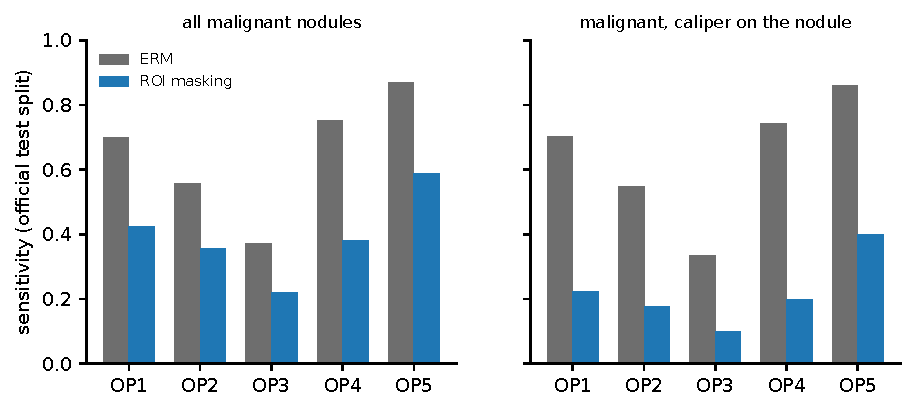
\includegraphics[width=\linewidth]{figures/op_thyroid.pdf}
\caption{Thyroid, official patient-disjoint test split: sensitivity of ERM and of the masked model at five
validation-fixed operating points, for all malignant nodules (left) and for the \sFiveNConf{} malignant nodules with a
caliper on the nodule (right; post hoc subgroup, exploratory).}\label{fig:op}\end{figure}
\begin{table}[H]\centering\scriptsize
\caption{Other natural test sets at OP2 (validation specificity $\ge0.80$), mask $-$ ERM, crossed CIs.}\label{tab:opother}
\begin{tabular}{lcccc}\toprule
Test set & Conflicting positives & $\Delta$ sensitivity & $\Delta$ specificity & $\Delta$ sensitivity, conflicting \\\midrule
Dermoscopy BCN & 1832 & $+0.017$ [$-0.003, +0.036$] & $-0.110$ [$-0.135, -0.079$] & $+0.019$ [$-0.004, +0.042$] \\
Dermoscopy HAM & 808 & $-0.062$ [$-0.110, -0.015$] & $+0.092$ [$+0.064, +0.121$] & $-0.055$ [$-0.104, -0.007$] \\
Dermoscopy MSK & 492 & $-0.074$ [$-0.127, -0.026$] & $+0.083$ [$+0.064, +0.110$] & $-0.094$ [$-0.149, -0.044$] \\
Capsule & 38 & $+0.140$ [$+0.082, +0.222$] & $+0.041$ [$-0.029, +0.107$] & $+0.022$ [$-0.041, +0.123$] \\
\bottomrule\end{tabular}
\end{table}

\begin{table}[H]\centering\scriptsize
\caption{Clinical metrics on the natural test sets (seed means; threshold at maximal balanced accuracy on validation data).}\label{tab:clin}
\begin{tabular}{lccccccc}\toprule
Test set & Arm & AUROC & AUPRC & Brier & ECE & Sensitivity & Specificity \\\midrule
Capsule (held-out frames) & ERM & 0.889 & 0.897 & 0.130 & 0.042 & 0.770 & 0.844 \\
 & mask & 0.967 & 0.971 & 0.069 & 0.029 & 0.856 & 0.933 \\
 & balanced & 0.881 & 0.889 & 0.136 & 0.051 & 0.757 & 0.838 \\
ISIC, BCN held out & ERM & 0.786 & 0.587 & 0.238 & 0.279 & 0.842 & 0.521 \\
 & mask & 0.761 & 0.564 & 0.287 & 0.330 & 0.842 & 0.443 \\
 & balanced & 0.782 & 0.587 & 0.229 & 0.260 & 0.835 & 0.509 \\
ISIC, HAM held out & ERM & 0.752 & 0.355 & 0.161 & 0.233 & 0.575 & 0.789 \\
 & mask & 0.782 & 0.396 & 0.138 & 0.199 & 0.569 & 0.831 \\
 & balanced & 0.751 & 0.350 & 0.154 & 0.225 & 0.495 & 0.845 \\
ISIC, MSK held out & ERM & 0.770 & 0.477 & 0.171 & 0.160 & 0.600 & 0.790 \\
 & mask & 0.785 & 0.497 & 0.149 & 0.120 & 0.587 & 0.823 \\
 & balanced & 0.767 & 0.464 & 0.175 & 0.165 & 0.628 & 0.759 \\
Thyroid (official split) & ERM & 0.735 & 0.604 & 0.209 & 0.088 & 0.699 & 0.653 \\
 & mask & 0.731 & 0.629 & 0.215 & 0.119 & 0.424 & 0.856 \\
 & balanced & 0.714 & 0.580 & 0.220 & 0.115 & 0.707 & 0.612 \\
\bottomrule\end{tabular}
\end{table}


\subsection{Replication breadth}
Table~\ref{tab:breadth}. The crossover's interval lies above zero for \sFiveNFrozenPos{} of \sFiveNFrozen{} frozen
encoder--cohort pairs (DINOv2 at three sizes, MedSigLIP, ConvNeXt); the exception is DermLIP. Among end-to-end
fine-tuned networks it replicates in \sFiveNFtPos{} of \sFiveNFt{} (dermoscopy hair, thyroid ViT-S, capsule); the
thyroid ResNet-50 and the ovary ResNet-50 are not significant, and the ovary network barely learns the task, so that
null is uninformative. On \textbf{new patients} --- ISIC 2020, \sFiveExtImages{} images from \sFiveExtPatients{}
patients, patient-disjoint folds, hair masks from a segmenter trained only on ISIC 2019 and frozen before any ISIC 2020
image was scored --- masking harms with hair on the lesion (\sFiveExttrapA) and helps with hair beside it
(\sFiveExttrapB); the crossover is \sFiveExtX{} (registered claim X1, supported).
\begin{table}[H]\centering\scriptsize
\caption{Replication breadth of the real-artifact crossover (crossed CIs).}\label{tab:breadth}
\begin{tabular}{lccc}\toprule
Cohort & Encoder & Training & Crossover [95\% CI] \\\midrule
Dermoscopy hair & DINOv2 ViT-S/14 & frozen & $+0.163$ [$+0.130, +0.195$] \\
Dermoscopy hair & DINOv2 ViT-B/14 & frozen & $+0.147$ [$+0.111, +0.185$] \\
Dermoscopy hair & DINOv2 ViT-L/14 & frozen & $+0.153$ [$+0.110, +0.195$] \\
Dermoscopy hair & DermLIP & frozen & $+0.014$ [$-0.037, +0.063$] \\
Thyroid & DINOv2 ViT-S/14 & frozen & $+0.247$ [$+0.205, +0.288$] \\
Thyroid & DINOv2 ViT-B/14 & frozen & $+0.239$ [$+0.196, +0.280$] \\
Thyroid & DINOv2 ViT-L/14 & frozen & $+0.263$ [$+0.218, +0.307$] \\
Thyroid & MedSigLIP-448 & frozen & $+0.195$ [$+0.153, +0.238$] \\
Thyroid & ConvNeXt-384 & frozen & $+0.275$ [$+0.231, +0.320$] \\
Ovary & DINOv2 ViT-S/14 & frozen & $+0.296$ [$+0.208, +0.384$] \\
Ovary & DINOv2 ViT-B/14 & frozen & $+0.170$ [$+0.087, +0.252$] \\
Ovary & DINOv2 ViT-L/14 & frozen & $+0.207$ [$+0.127, +0.286$] \\
Ovary & MedSigLIP-448 & frozen & $+0.178$ [$+0.109, +0.248$] \\
Capsule & DINOv2 ViT-S/14 & frozen & $+0.370$ [$+0.325, +0.415$] \\
Capsule & DINOv2 ViT-B/14 & frozen & $+0.377$ [$+0.327, +0.426$] \\
Capsule & DINOv2 ViT-L/14 & frozen & $+0.417$ [$+0.369, +0.464$] \\
Capsule & MedSigLIP-448 & frozen & $+0.335$ [$+0.286, +0.383$] \\
Capsule & ConvNeXt-384 & frozen & $+0.320$ [$+0.268, +0.372$] \\
Dermoscopy hair & ResNet-50 & fine-tuned & $+0.143$ [$+0.054, +0.232$] \\
Thyroid & ResNet-50 & fine-tuned & $+0.063$ [$-0.022, +0.144$] \\
Thyroid & ViT-S & fine-tuned & $+0.122$ [$+0.039, +0.211$] \\
Capsule & ResNet-50 & fine-tuned & $+0.606$ [$+0.495, +0.716$] \\
Ovary & ResNet-50 (15 clusters) & fine-tuned & $+0.058$ [$-0.062, +0.179$] \\
Dermoscopy hair, ISIC 2020 (external) & DINOv2 ViT-B/14 & frozen, new patients & $+0.250$ [$+0.174, +0.327$] \\
\bottomrule\end{tabular}
\end{table}

\begin{figure}[H]\centering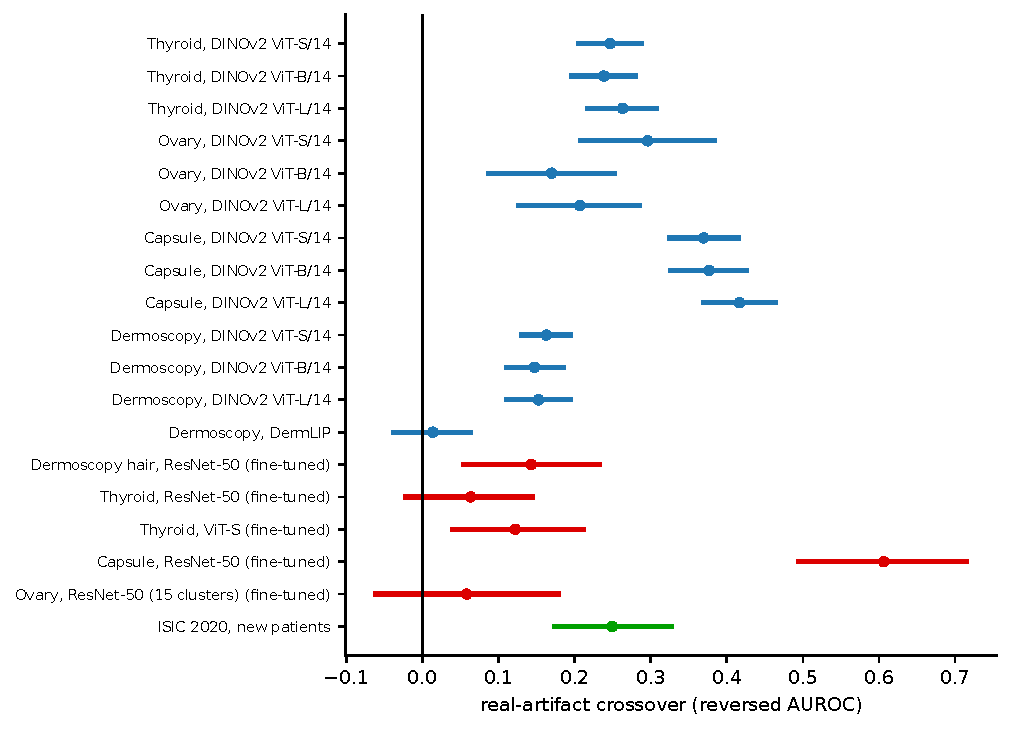
\includegraphics[width=0.8\linewidth]{figures/breadth_forest.pdf}
\caption{Crossover across encoders, scales, fine-tuned networks (red) and new patients (green); crossed 95\% CIs.}
\label{fig:breadth}\end{figure}

\subsection{The DermLIP exception}
With DermLIP, masking harms at both hair locations (Trap~A \sFiveDermmasktrapAtestrev, Trap~B
\sFiveDermmasktrapBtestrev). Two measurements explain it. First, masking costs DermLIP disease signal wherever the hair
lies: clean-test AUROC changes by \sFiveDermmasktrapAclean{} and \sFiveDermmasktrapBclean. Second, the pixel part of
its hair shortcut is small at both locations (oracle hair inpainting \sFiveDerminpainttrapAtestrev{} and
\sFiveDerminpainttrapBtestrev), whereas group balancing, which also removes correlates of hair, gains
\sFiveDermbalancedtrapAtestrev{} and \sFiveDermbalancedtrapBtestrev: DermLIP carries the hair shortcut mostly through
correlates that masking does not remove at either location. The theory anticipates this from the clean and correlated
AUROC alone: predicted crossover \sFiveDermPred, observed \sFiveDermObs.

\subsection{The theory, judged by held-out error}
Table~\ref{tab:theory} and Figure~\ref{fig:theory}. Over \sFiveTN{} primary cells the theory predicts the reversed
AUROC --- never used in fitting --- with mean absolute error \sFiveTMae{} (Pearson $r$ \sFiveTR; \sFiveTWithin{}
within 0.05), against \sFiveTMaeSym{} for the symmetric-reversal heuristic and \sFiveTMaeClean{} for ``reversed =
clean''. It gets the sign of all \sFiveTTwoN{} real-trap crossovers right (MAE \sFiveTTwoMae) and of \sFiveTTwoFt{}
fine-tuned crossovers, and the sign of \sFiveTThreeSign{} of \sFiveTThreeN{} controlled-sweep gains (heuristic:
\sFiveTThreeSymSign). The account is simple: a model's reliance on an artifact is fixed by the ratio of artifact to disease
signal it sees; masking lowers the disease signal (less context) and leaves an in-ROI artifact's signal intact, so it
raises that ratio exactly when the artifact is inside the ROI.
\begin{table}[H]\centering\scriptsize
\caption{Held-out prediction of the reversed-test AUROC (never used in fitting): the two-parameter theory fitted to each cell's clean and correlated AUROC, against two parameter-free heuristics.}\label{tab:theory}
\begin{tabular}{lccccc}\toprule
Cells & Predictor & $n$ & MAE & Pearson $r$ & within 0.05 \\\midrule
Primary cells (ERM, mask) & linear-Gaussian theory & 136 & 0.052 & 0.914 & 66\% \\
 & heuristic: symmetric reversal & 136 & 0.129 & 0.743 & 40\% \\
 & heuristic: reversed = clean & 136 & 0.237 & 0.550 & 18\% \\
All ERM-head arms & linear-Gaussian theory & 598 & 0.036 & 0.933 & 79\% \\
 & heuristic: symmetric reversal & 598 & 0.076 & 0.823 & 65\% \\
 & heuristic: reversed = clean & 598 & 0.151 & 0.584 & 40\% \\
Fine-tuned (outside assumptions) & linear-Gaussian theory & 12 & 0.027 & 0.980 & 92\% \\
\bottomrule\end{tabular}
\end{table}

\begin{figure}[H]\centering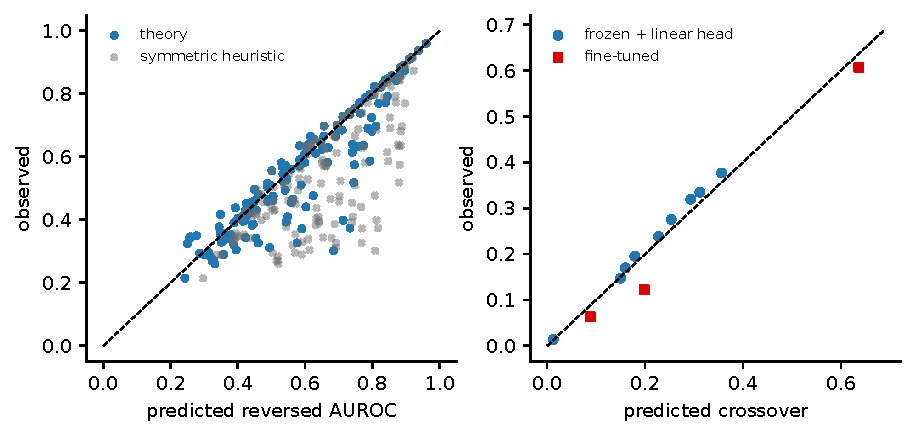
\includegraphics[width=\linewidth]{figures/theory_prediction.pdf}
\caption{Left: predicted versus observed reversed AUROC (theory, blue; symmetric heuristic, grey). Right: predicted
versus observed real-trap crossover (frozen encoders, blue; fine-tuned, red).}\label{fig:theory}\end{figure}

\section{What failed or changed}
\begin{itemize}[leftmargin=*]\itemsep1pt
\item \textbf{Natural test sets}: N3 holds in three of five; HAM goes the other way and capsule is inconclusive. With
the corrected bootstrap, masking's gain on easy thyroid pairs and U-MtE's gain over masking on hard thyroid pairs are no
longer significant.
\item \textbf{The thyroid subgroup} is a post hoc subgroup; its test was registered only after its AUROC result was
known. Its interval is now the corrected one.
\item \textbf{Fine-tuning}: thyroid ResNet-50 is not significant; the archived ovary ResNet-50 run could not be
regenerated (no saved predictions) and is withdrawn; the 15-cluster ovary re-run is uninformative.
\item \textbf{DermLIP}: no crossover; explained, and predicted by the theory, but still an exception.
\item \textbf{Absolute performance} is below task-specific fine-tuned models on thyroid (frozen DINOv2 with a linear head
reaches a clean AUROC of \sFiveThyAucerm{} on the official split).
\end{itemize}

\section{Conclusion}
\textbf{Supported.} On unaltered data masking harms the shortcut-conflicting cases in three of five test sets and lowers
thyroid sensitivity at every validation-fixed operating point (registered decision rule met). The crossover replicates
across encoder families and sizes, in three of five fine-tuned networks and on new patients. A two-parameter theory
predicts held-out reversed AUROC far better than heuristics and anticipates the DermLIP exception.
\textbf{Qualified.} The \sFiveNConf-nodule subgroup is exploratory confirmation. \textbf{Not supported.} Harm on natural
HAM and capsule test sets; the crossover for DermLIP and for two fine-tuned networks.

\section{Questions for the supervisor}
\begin{enumerate}\itemsep1pt
\item Is a sensitivity loss on one patient-disjoint split (thyroid) enough for the clinical claim in the abstract, or
should the abstract lead with the AUROC on shortcut-conflicting cases?
\item Should the theory be a main contribution (with its held-out error as evidence) or a supporting section?
\item Is ISIC 2020 enough external validation, given that it is the same modality and artifact as the main dermoscopy
analysis?
\end{enumerate}

\section{Next stage}
Stage~6 turns to what to do instead of masking (the decision guide, with its remedies tested in the primary family),
the blinded image audit prepared for a clinician, the limitations, the paper itself, the CLAIM checklist and the
submission statements.

\bibliographystyle{plainnat}
\bibliography{../common/references}
\end{document}
